% 固定来源PDF印刷页52第5题三条直线斜率关系的矢量示意重绘。
% 仅表达斜率的正负与大小次序，不表示题设给定的精确坐标。
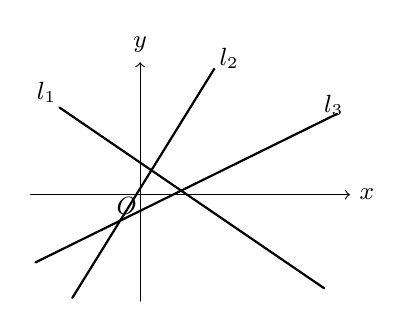
\begin{tikzpicture}[x=.82cm,y=.82cm,font=\small,line cap=round,line join=round]
  \draw[->] (-1.7,0)--(3.25,0) node[right] {$x$};
  \draw[->] (0,-1.65)--(0,2.05) node[above] {$y$};
  \draw[thick] (-1.25,1.35)--(2.85,-1.45);
  \draw[thick] (-1.05,-1.6)--(1.15,1.95);
  \draw[thick] (-1.62,-1.05)--(3.05,1.25);
  \node[above left] at (-1.15,1.28) {$l_1$};
  \node[above right] at (1.08,1.8) {$l_2$};
  \node[above right] at (2.7,1.08) {$l_3$};
  \node[below left,inner sep=1pt] at (0,0) {$O$};
\end{tikzpicture}
